\documentclass{anstrans}
%%%%%%%%%%%%%%%%%%%%%%%%%%%%%%%%%%%
\title{Energy Expansion in Response Matrix Methods Using the Karhunen-Lo\`{e}ve Transform}
\author{Richard L. Reed, Jeremy A. Roberts}

\institute{
Mechanical and Nuclear Engineering, Kansas State University, Manhattan, KS
}

\email{blkpawn@k-state.edu \and jaroberts@k-state.edu}

% Optional disclaimer: remove this command to hide
%\disclaimer{Notice: This manuscript is a work of fiction. Any resemblance to
%actual articles, living or dead, is purely coincidental.}

%%%% packages and definitions (optional)
\usepackage{graphicx} % allows inclusion of graphics
\usepackage{booktabs} % nice rules (thick lines) for tables
\usepackage{microtype} % improves typography for PDF
\usepackage{xcolor}

\graphicspath{{figures/}} % Specifies the directory where pictures are stored

\newcommand{\SN}{S$_N$}
\renewcommand{\vec}[1]{\bm{#1}} %vector is bold italic
\newcommand{\vd}{\bm{\cdot}} % slightly bold vector dot
\newcommand{\grad}{\vec{\nabla}} % gradient
\newcommand{\ud}{\mathop{}\!\mathrm{d}} % upright derivative symbol

\begin{document}
%%%%%%%%%%%%%%%%%%%%%%%%%%%%%%%%%%%%%%%%%%%%%%%%%%%%%%%%%%%%%%%%%%%%%%%%%%%%%%%%
\section{Introduction}

This paper presents a new representation of the energy variable for use in
response matrix methods, and, in particular, the eigenvalue response matrix
method (ERMM).  ERMM solves the reactor eigenvalue equation,
\begin{equation}
  \mathcal{T} \phi(\bm{\rho}) =
    \frac{1}{k} \mathcal{F} \phi(\bm{\rho}) \, ,
  \label{eq:global}
\end{equation}
where $\bm{\rho}$ contains the relevant phase space (i.e., $\mathbf{r}$, $E$, and $\Omega$),
by decomposing the domain into independent nodes linked through approximate
boundary conditions based on truncated, orthogonal basis expansions.  Proper
selection of orthogonal bases in each phase space variable is critical to
success of ERMM in real-world applications.  In short, basis sets that capture
high-fidelity transport solutions with low-order expansions are ideal. The rest
of this paper provides a short review of ERMM based on presentation of Ref.
\cite{RobertsSerment}, followed by the presentation of a new, highly successful
energy basis for use in ERMM based on the Karhunen-Lo\`{e}ve transform and its
application to an illustrative problem.

\section{Methods}

\subsection{Overview of ERMM}

Suppose the global problem of Eq. \ref{eq:global} is defined over a
volume, $V$, which can be decomposed into $N$ disjoint, nodal subvolumes,
$V_i$, that satisfy $V = V_1 \bigcup V_2 \bigcup \ldots \bigcup V_N$.
Then a local transport problem for the $i$th node is defined
\begin{equation}
  \mathcal{T} \phi(\bm{\rho}_i) =
    \frac{1}{k} \mathcal{F} \phi(\bm{\rho}_i) \, ,
  \label{eq:local}
\end{equation}
subject to the incident current boundary condition
\begin{equation}
  J^{\mathrm{}}_{-} (\bm{\rho}_{is}) =
    J^{\mathrm{global}}_{-}(\bm{\rho}_{is}) \, ,
  \label{eq:localbc}
\end{equation}
where $J_{-} (\bm{\rho}_{is}) $ is the incident angular current on
surface $s$.  Because the global currents are not known
{\it a priori}, the local boundary currents are represented as a truncated
expansion in an
orthogonal basis, $P_m(\bm{\rho}_{is}), \,\,\, m = 0, \, 1, \, \ldots$,
defined over the surface phase space $\bm{\rho}_{is}$.
% is used subject to
% \begin{equation}
%    \int d\rho_{is} P_m(\bm{\rho}_{is})P_n(\bm{\rho}_{is}) = \delta_{mn} \, .
% \end{equation}
By solving Eq. \ref{eq:local} subject to the $m$th order
incident condition
\begin{equation}
 J^{}_{-} (\bm{\rho}_{is}) = P_m(\bm{\rho}_{is}) \,
\end{equation}
on one surface, $s$, and vacuum elsewhere,
a response function is defined as
\begin{equation}
       r^{ms}_{im's'} = \int d\rho_{is'} P_{m'}(\bm{\rho}_{is'})
        J_{+} (\bm{\rho}_{is'}) \, ,
\label{eq:responsefunction}
\end{equation}
where $J^+$ is the outgoing angular current.  The
response function $r^{ms}_{im's'}$
is the $m'$th order current response out of
surface $s'$ due to an $m$th order incident current on
surface $s$.
%
% A response equation is defined
% \begin{equation}
%  \mathcal{T} \phi_{i}^{ms} (\bm{\rho}_i) =
%    \frac{1}{k} \mathcal{F} \phi_{i}^{ms} (\bm{\rho}_i)
%  \label{eq:rfequation}
% \end{equation}
% subject to the incident condition
% \begin{equation}
%  J^{}_{-} (\bm{\rho}_{is}) = P_m(\bm{\rho}_{is})
% \end{equation}
% on one surface, $s$, and vacuum elsewhere.
% By solving Eq. \ref{eq:rfequation} for the outgoing
% currents, $J_{+}$,
% a response function is defined as
% \begin{equation}
%        r^{ms}_{im's'} = \int d\rho_{is'} P_{m'}(\bm{\rho}_{is'})
%         J_{+} (\bm{\rho}_{is'}) \, ,
% \label{eq:responsefunction}
% \end{equation}
% which represents the $m'$th order current response out of
% surface $s'$ due to an $m$th order incident current on
% surface $s$.
By expressing the incident and outgoing currents, $J_{\mp}$, as truncated
expansions in the basis, global neutron balance can be represented by the
response matrix equation
\begin{equation}
  \mathbf{M}\mathbf{R}(k)\mathbf{J_-}  = \lambda \mathbf{J_-} \, ,
\label{eq:erme}
\end{equation}
where $\mathbf{R}$ contains response functions, $\mathbf{J}_{-}$ contains the
incident angular current expansion coefficients, $\mathbf{M}$ is a matrix that
redirects outgoing currents as incident currents of neighbors, and $\lambda$ is
an eigenvalue that approaches unity as $k$ approaches its correct value. The
$k$-eigenvalue is computed iteratively by alternately solving for
$\mathbf{J}_{-}$ and updating $k$ based on balance \cite{RobertsSerment}.

\subsection{Expanding in Energy}

Historically, response matrix implementations have used full multigroup
approximation in energy, which leads to full consistency between local transport
solutions and the global response matrix solution with respect to energy. Most
recent work on response matrix methods has used relatively coarse multigroup
libraries, ranging from a few groups \cite{ishii2009tdd} to seven groups
\cite{forget2006tdh}. However, more realistic analyses require dozens of groups
or more, and a basis that can capture many-group fidelity with many---ideally an
order of magnitude---fewer energy degrees of freedom would be of substantial
value.

Recent work investigated the use of discrete Legendre polynomials (DLP) and
modified DLP (mDLP) for expansion in energy \cite{Roberts2014}.  The mDLP basis
modifies the DLP basis by superimposing a ``shape'' vector on each basis vector.
 The shape vector is chosen to be representative of the vector subject to
expansion, i.e., the energy-dependent angular current.  Previously, a spatially
averaged energy spectrum from a representative lattice problem has been used
with moderate success \cite{Roberts2014}.

\subsection{The  Karhunen-Lo\`{e}ve Energy Basis}

Although mDLP represents one way in which to build physics into an energy basis,
 a more powerful approach is to use the Karhunen-Lo\`{e}ve transform (KLT)
\cite{Dony2001}. The method was originally conceived as a method of image
compression but has been adapted to generic data compression \cite{Buchan2013}
and model reduction \cite{Sirovich1987}.

The KLT is based on a small set of vectors representative of a much larger
problem space. These vectors, called ``snapshots,'' are used to construct a set
of eigenvectors such that the projection of a generated basis function onto the
expanded function is maximized \cite{Sirovich1987}. Thus, by construction, the
KLT
produces the most efficient set of basis vectors to approximate a given data
set, in the sense of the maximum amount of data retained.

To generate the basis functions, a data matrix, $\mathbf{D}$, is formed by
combining $M$ snapshot vectors, each of length $N$, as an $M \times N$ matrix
\cite{Meyer2002}.  Then the $N \times N$ matrix $\mathbf{B}$ is defined as
\begin{equation}
 \mathbf{B} = \mathbf{D}^{T}\mathbf{D} \, .
\end{equation}
Let $\mathbf{b}_j$ and $\lambda_j$ represent the eigenvectors and
eigenvalues of $\mathbf{B}$, i.e.,
\begin{equation}
 \mathbf{Bb}_j = \lambda_j \mathbf{b}_j \,  \quad \text{where} \quad \lambda_j > \lambda_{j+1} \, , \forall j \, .
\end{equation}
%ordered so that $\lambda_j > \lambda_{j+1}$ for all $j$.
The eigenvectors are then multiplied by the data matrix to form the basis vectors, $\mathbf{y}_j$, i.e.,
\begin{equation}
 \mathbf{y}_j = \mathbf{D}\mathbf{b}_j \, ,
\end{equation}
which are subsequently orthogonalized.  Then approximate representation of an arbitrary $N$-vector, $\mathbf{f}$, in the basis is
\begin{equation}
 \mathbf{f} \approx \sum_j a_j \mathbf{y}_j \, \quad \text{where} \quad a_j = \mathbf{f}^T \mathbf{y}_j \, .
\end{equation}
% where
% \begin{equation}
%  a_j = \mathbf{f}^T \mathbf{y}_j \, .
% \end{equation}

When used as an energy basis within ERMM, KLT snapshots are energy group-
dependent flux or current vectors from several spatial cells within one or more
representative models.  Similar to use of simple, but representative, spatial
models for self-shielding in lattice physics calculations, equally simple,
inexpensive models can be used to generate snapshot vectors for computing a KLT
basis.  In the following section, specific approaches used for defining these
simplified models and extracting snapshots from them are described.

\section{Results and Analysis}

\subsection{Test Problem}

For use as an illustrative test case, a 10-pin, UO$_2$-MOX slab assembly model
was developed (referred to as the test problem). Fuel for the left five pins was
UO$_2$, while the right five pins were composed of MOX. Boundary conditions on
either side of the model were reflective. The cross section library used was
generated with SCALE 5.1 in the SCALE 44-group format \cite{Scale}.

Fuel pins were 1.08 cm thick with 0.10 cm of moderator on each side. The
baseline pin cell discretization consisted of 22 mesh cells of fuel enclosed by
three mesh cells of moderator on either side, and, thus, each pin cell provides
28 energy-dependent snapshots. A 16-angle, double Gauss-Legendre quadrature and
a diamond-difference spatial discretization were used for all calculations
\cite{Roberts2014}.

A current-conserving, first-order, angular expansion based on Jacobi polynomials
 \cite{Roberts2014} was used throughout.  Because the problem is 1-D, the nodal
boundary currents have no spatial dependence (and so spatial expansions are
unnecessary). For energy, DLP, mDLP, and KLT bases were explored as a function
of the energy expansion order.

All calculations were performed with the {\tt Serment} parallel response matrix
code \cite{RobertsSerment}, which links to the {\tt Detran} deterministic
transport code \cite{RobertsDetran}. {\tt Detran} implements discrete ordinates,
method of characteristics, and diffusion approximations, along with several
advanced solvers developed specifically for use in response function generation.
For this paper, only its discrete ordinates capabilities were used.

\subsection{Generation of Snapshots}

\begin{table*}
  \centering
  \caption{Summary of models used for snapshot generation}
  \begin{tabular}{c | l}\toprule
    Abbreviation    & Model to generate snapshots \\ \midrule
    MOX Pin         & MOX pin only \\
    UO$_2$ Pin      & UO$_2$ pin only \\
    UO$_2$-Mod-MOX  & 1 UO$_2$ pin + 1 moderator pin + 1 MOX pin (with reflecting BC) \\
    3 Pin Combined  & 1 UO$_2$ pin, 1 MOX pin, 1 moderator pin modeled separately then combined \\
    1 pin           & Repeating array of 1 UO$_2$ and 1 MOX pin \\
    2 pin           & Repeating array of 2 UO$_2$ and 2 MOX pins \\
    6 pin           & Repeating array of 6 UO$_2$ and 6 MOX pins \\
    10 pin          & Repeating array of 10 UO$_2$ and 10 MOX pins (i.e., the test problem)\\
    14 pin          & Repeating array of 14 UO$_2$ and 14 MOX pins \\
    \bottomrule
  \end{tabular}
  \label{tab:snapshots}
\end{table*}

Ideally, with any form of model reduction, computational effort needed to solve a given problem is reduced, so a basis set that is quickly computed is sought. As such, generating snapshots for the KLT was a primary focus for this work.  Because the test problem and snapshot models studied are comparatively small, timing studies would provide little insight.  However, for larger, 2-D or 3-D models (e.g.,
assemblies or full cores), the snapshot models (e.g., pin cells or sub-assemblies) are expected to be orders of magnitude less computationally expensive than the full model of interest.

The test problem is a 1-D approximation to the junction between a UO$_2$ and MOX assembly.  Therefore, a number of small, representative subproblems are natural choices for generation of snapshots.  Models studied in this paper are summarized in Table \ref{tab:snapshots} but warrant discussion.  The simplest approach for generating snapshots is to model each pincell individually, subject to reflecting boundary conditions on all surfaces, and to extract snapshots (i.e., energy-dependent vectors in distinct spatial cells) from an individual pincell or to combine snapshots from both pincell models.  A larger energy space is obtained if a single model includes more than one pin (fuel or moderator), in various arrangements.  Here, an effectively $1\times 1$ (infinite lattice of one UO$_2$ and one MOX pin; abbreviated as the ``1-pin model''), $2 \times 2$, $6 \times 6$, $10 \times 10$, and $14 \times 14$ model were studied.  The $10 \times 10$ model is exactly the test problem of interest and should be expected to yield snapshots that represent the true multigroup solution with the lowest-order energy expansion.

Because the test problem reference solution is a full transport approximation, boundary currents generally exhibit coupled angle-energy dependence.  By including
snapshots that incorporate angular information, the resulting KLT basis may outperform snapshots based on the scalar flux, $\phi$, alone.  To do so, snapshots were taken of either the energy-dependent net current, $J_{\text{net}}$, or partial current, $J_{\text{left}}$.  The direction for the partial current is arbitrary because the snapshot models are symmetric. Because the diamond-difference discretization produces only one spatial unknown per cell, the snapshot generation approach
used provides either one (just $\phi$) or two ($\phi$ and either $J_{\text{left}}$ or $J_{\text{net}}$) snapshots per spatial cell.

\subsection{Comparison of Bases}

In this section, the methods described were applied to the test problem.
A typical goal of reactor analysis is to compute pin fission densities
(or powers) with sub-$1\%$ errors.  In order to add an additional
buffer, the goal of this work is to minimize the energy expansion order
required to achieve sub-$0.1\%$ maximum relative fission density errors.
The reference solution in all cases is a full multigroup response matrix solution
with the same angular expansion used throughout; in other words, any
changes in the solution observed when using various energy bases is a
function of the energy basis alone.

\begin{figure}[htb]
 \centering
 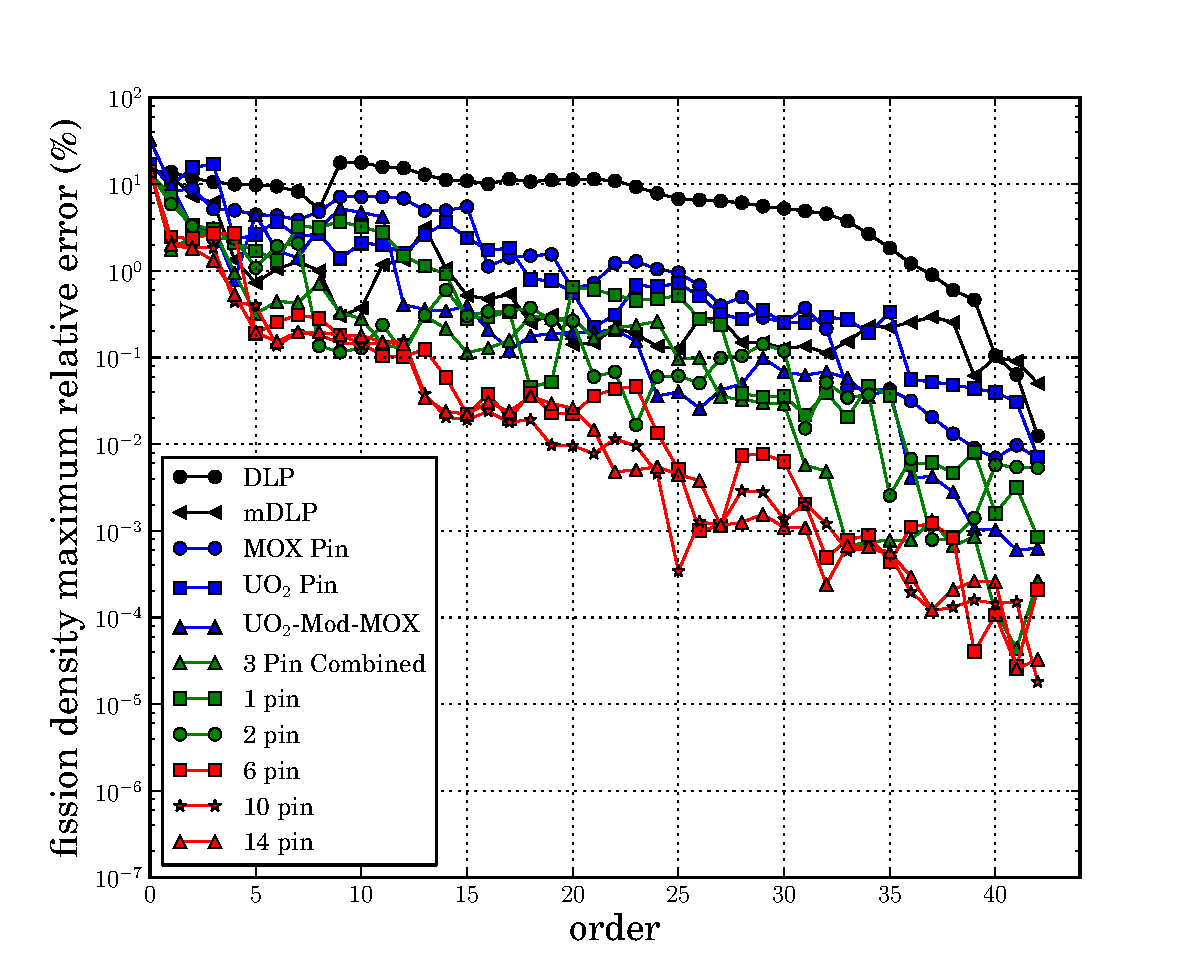
\includegraphics[trim=.5cm .25cm 1.5cm 1.25cm, clip=true, totalheight=0.28\textheight]{phi}
 \caption{Relative error using only $\phi$ data}
 \label{fig:phi}
\end{figure}

\begin{figure}[htb]
 \centering
 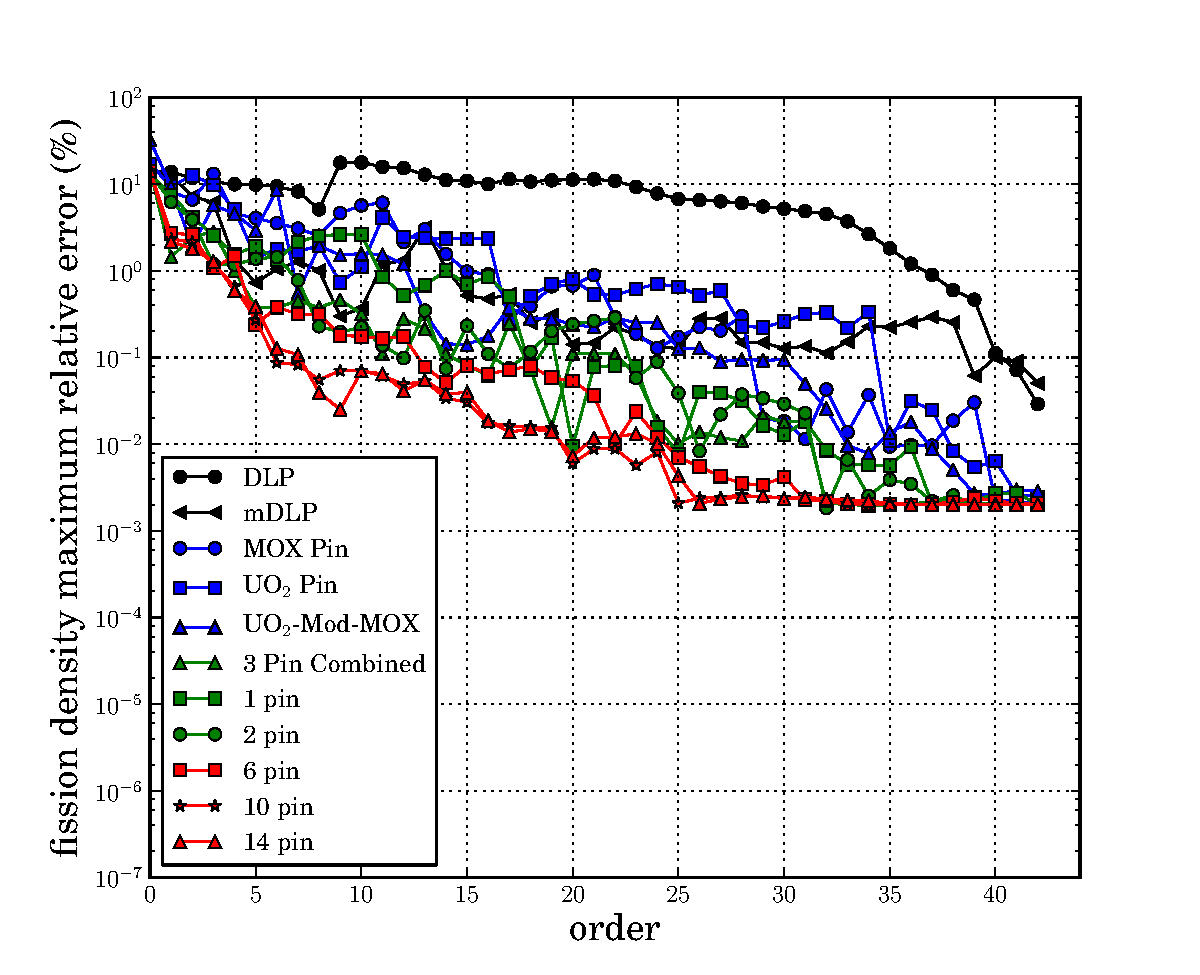
\includegraphics[trim=.5cm .25cm 1.5cm 1.25cm, clip=true, totalheight=0.28\textheight]{netcurrent}
 \caption{Relative error using $\phi$ and $J_{\text{net}}$ data}
 \label{fig:totalcurrent}
\end{figure}

\begin{figure}[htb]
 \centering
 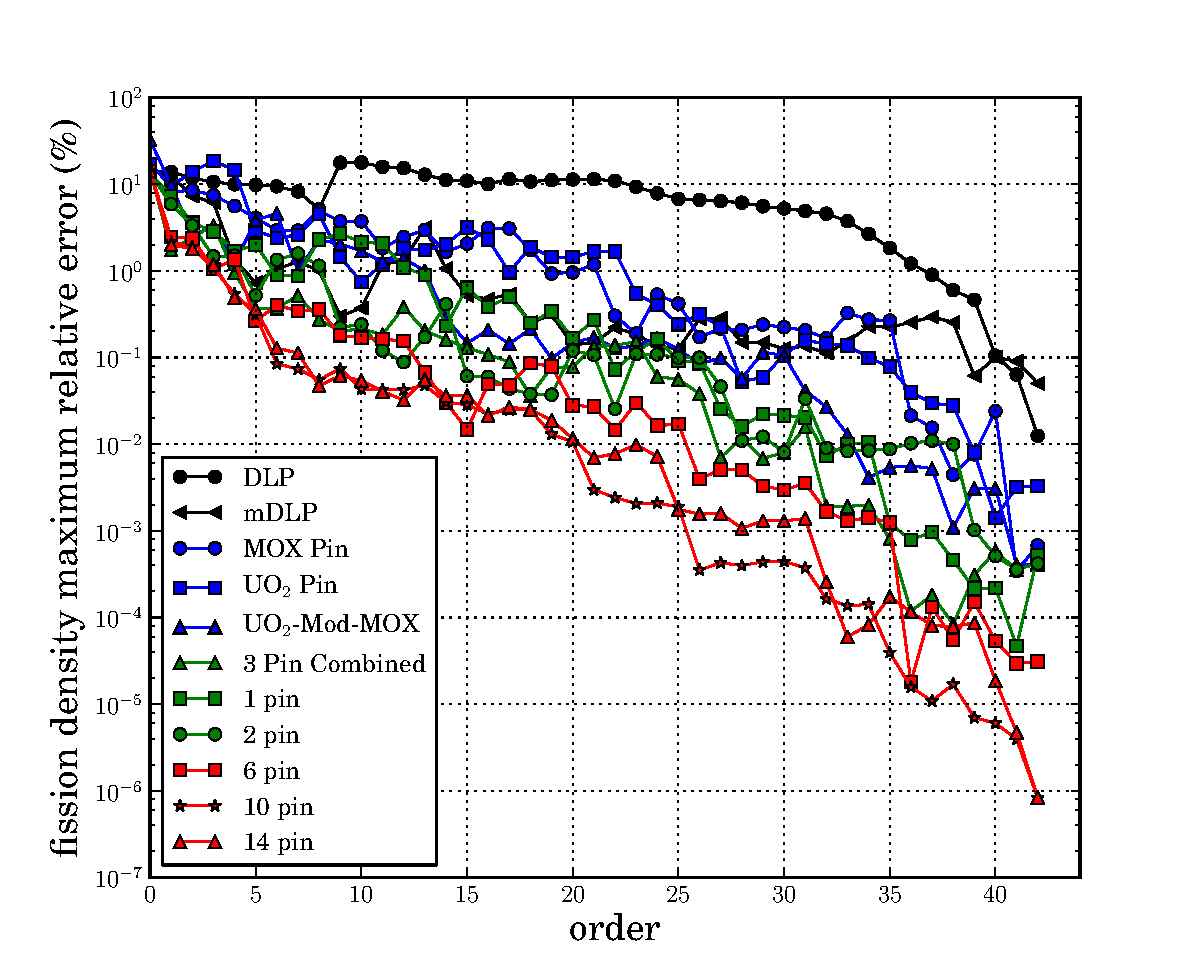
\includegraphics[trim=.5cm .25cm 1.5cm 1.25cm, clip=true, totalheight=0.28\textheight]{partialcurrent}
 \caption{Relative error using $\phi$ and $J_{\text{left}}$ data}
 \label{fig:partialcurrent}
\end{figure}

The first three figures compare the various bases.  Each of the curves except for `DLP' and `mDLP' was generated using the KLT basis with distinct snapshot data. The mDLP results represent the best case previously observed \cite{Roberts2014}.  As shown in Figures \ref{fig:phi}, \ref{fig:totalcurrent}, and \ref{fig:partialcurrent}, all KLT bases outperformed DLP.  Snapshots generated from both UO$_2$ and MOX perform as well or better than mDLP, while single pin models do not. The 43rd order is excluded from all curves because the results are exact to within the convergence tolerance.

Figure \ref{fig:phi} shows results of using only scalar flux, $\phi$, as data for snapshots.  When using snapshots from models that closely resemble the test problem, relative error falls below the 0.1$\%$ threshold at around an energy order of 12.  The other models require an energy expansion order of at least 20, far from the goal of approximately five.

When the net current or partial current are included with the scalar flux, results are improved, as can be observed in Figures \ref{fig:totalcurrent} and \ref{fig:partialcurrent}.  The 10-pin snapshot model yields sub-0.1$\%$ fission density errors with just sixth order expansions when either net or partial current is included.  Most of the other smaller models still fall short of the goal of an order of magnitude reduction in required energy order; however, the 1-pin and 2-pin models perform reasonably well considering their simplicity.  For higher orders, the net current results appear to stagnate, which suggests that the partial current contributes more useful information to the KLT basis.  However, this is expected because the partial current better represents the boundary data being expanded, i.e., the angular current.

\subsection{Sensitivity to Snapshot Selection}

\begin{figure}[htb]
 \centering
 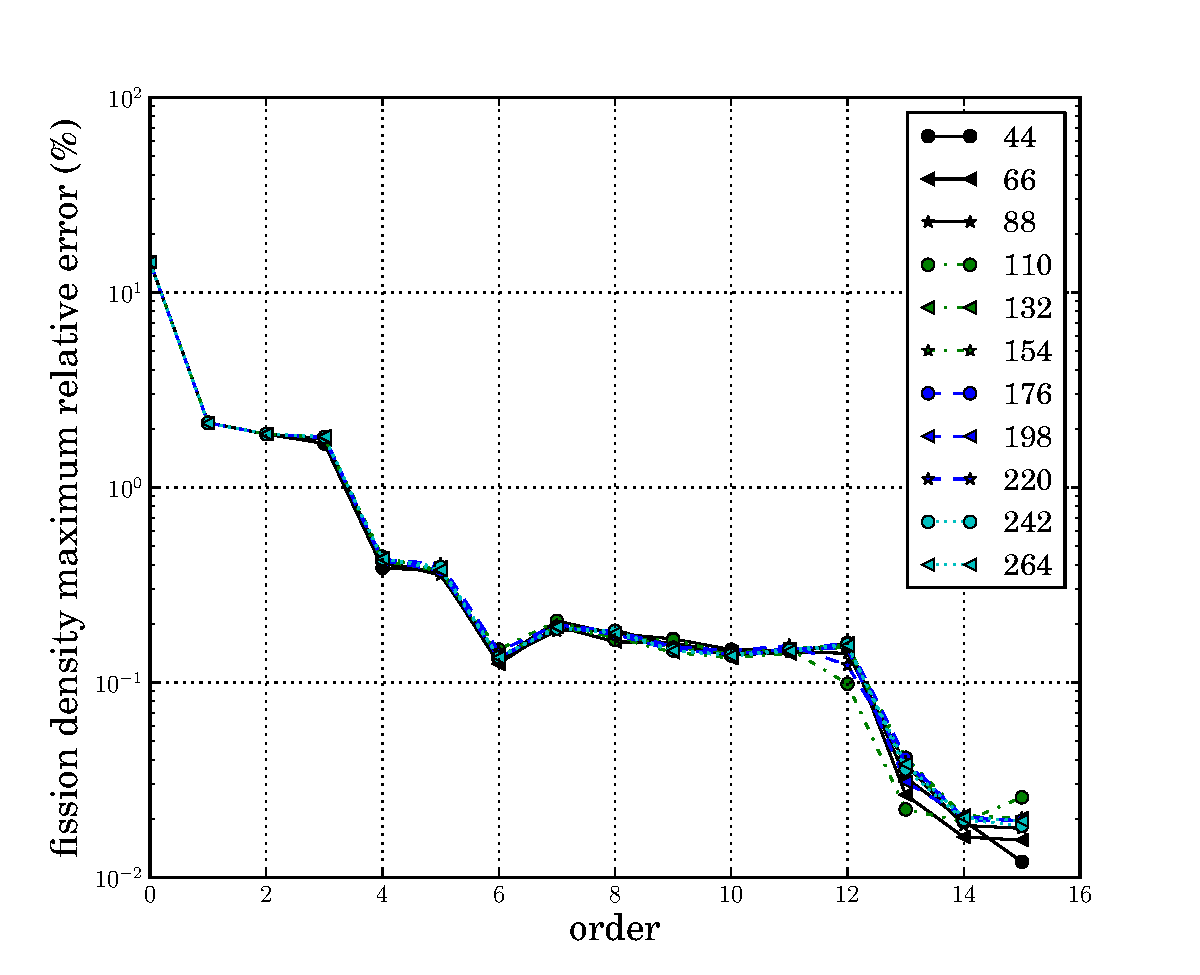
\includegraphics[trim=.5cm .25cm 1.5cm 1.25cm, clip=true, totalheight=0.28\textheight]{number}
 \caption{Relative error as a function of expansion order for various numbers of snapshots}
 \label{fig:number}
\end{figure}

To study sensitivity of  the KLT basis to selection of snapshots, the 10-pin model spatial discretization was varied to produce a greater or smaller number of spatial cells, and, hence, potential snapshots. It was found that mesh size has a relatively small effect on the efficacy of the generated basis set.  Additional snapshots from the same model will be exceedingly similar to the others, which will not add any additional information to the expansion.

In addition, the effect of using a variable number of snapshots from the baseline 10-pin model was studied, results of which are shown in Figure \ref{fig:number}.  The study selected evenly spaced snapshots from the 10-pin data (i.e., given 280 available snapshots, only every $x$th snapshot was used to generate the basis). The resulting impact is negligible.  In other words, inclusion of additional snapshots does not improve the results unless new snapshots are meaningfully distinct from the current set of snapshots.
Based on these results, all available snapshots were used to produce Figures \ref{fig:phi}--\ref{fig:partialcurrent}.
%
% Due to the results of the parametric studies, for the results depicted in Figures \ref{fig:phi}, \ref{fig:totalcurrent}, and \ref{fig:partialcurrent}, all of the produced data from the various models were used as snapshots for basis generation.

\section{Conclusion}

The KLT basis outperforms the mDLP and DLP bases for ERMM energy expansions because the KLT, by construction, maximizes the amount of information contained in low-order expansions. When using appropriate data for generating the basis, sufficient accuracy (i.e., sub-0.1\% maximum relative error in fission density) can be obtained with as few as one-tenth of the equivalent energy degrees of freedom used in a full multigroup approximation. The results are improved by including the net or partial current in generation of snapshots.

The results further suggest that adding more snapshots will improve the data only if the new snapshots are unique.  Thus, the inclusion of partial or net current snapshots improves results because the snapshots differ meaningfully from scalar flux snapshots.  Contrarily, the use of a greater number of snapshots from a finer spatial mesh yields diminishing improvement because the new snapshots become increasingly similar.  For most problems of interest, there exists a sufficiently large number of unique spatial regions for use in snapshot generation, and a key goal of ongoing work is to determine other variables (e.g, increased angle dependence) that can provide greater snapshot variety.

Other ongoing work aims to extend the use of KLT energy expansions to 2-D problems, for which the method is expected to yield similarly encouraging results.  Additionally, use of 44 group data in this work goes well beyond the typical few-group libraries typically employed in the response matrix literature, but future work will investigate use of $100+$ group libraries more typical of lattice physics.

%\section*{References}
\setlength{\baselineskip}{12pt}

\bibliographystyle{ans}
\bibliography{bibliography}
\end{document}